\documentclass[xcolor=dvipsnames
              %,handout
              ]{beamer} 

\usetheme{Madrid} 
%\setbeamertemplate{blocks}[shadow=false] 
\setbeamertemplate{navigation symbols}{} 
\setbeamertemplate{items}[square]
\setbeamertemplate{sections/subsections in toc}[square]

\definecolor{myblueend}{rgb}{0.058,0.132,0.42}
\definecolor{mybluemiddle}{rgb}{0.31,0.45,0.64}
\definecolor{mybluestart}{rgb}{0.17,0.28,0.48}
\definecolor{mygreen}{rgb}{0,0.7,0}
\definecolor{mylightgreen}{rgb}{0.7,1,0.7}
\definecolor{mylightblue}{rgb}{0.7,0.7,1}
\definecolor{mylightblack}{rgb}{0.7,0.7,0.7}
\definecolor{mylightred}{rgb}{1,0.7,0.7}
\definecolor{oproverblue}{RGB}{12,83,144}
\definecolor{oproveryellow}{RGB}{255,156,55}
\definecolor{mydarkgreen}{rgb}{0.17,0.48,0.28}
\definecolor{mydarkred}{rgb}{0.48,0.28,0.17}
\definecolor{grey}{rgb}{0.7,0.7,0.7}

%\setbeamercolor{palette primary}{fg=white,bg=mybluestart}
%\setbeamercolor{palette secondary}{fg=white,bg=mybluestart}
%\setbeamercolor{palette tertiary}{fg=white,bg=mybluestart}
%\setbeamercolor{palette quaternary}{fg=white,bg=mybluestart}
\setbeamercolor{palette primary}{fg=white,bg=oproverblue}
\setbeamercolor{palette secondary}{fg=white,bg=oproverblue}
\setbeamercolor{palette tertiary}{fg=white,bg=oproverblue}
\setbeamercolor{palette quaternary}{fg=white,bg=oproverblue}
\setbeamercolor{titlelike}{parent=palette quaternary}

\setbeamercolor{item}{fg=oproverblue}
\setbeamercolor{block title}{fg=white,bg=oproverblue}
\setbeamercolor{block title example}{fg=white,bg=oproveryellow}
%\setbeamercolor{block title alert}{fg=white,bg=mydarkred}

\usefonttheme{serif}

%%
%% TOOLS
%% 
\newcommand{\opensmt}{{\sc OpenSMT}\xspace}
\newcommand{\yices}{{\sc Yices}\xspace}
\newcommand{\mathsat}{{\sc MathSAT}\xspace}
\newcommand{\cvcfour}{{\sc CVC4}\xspace}
\newcommand{\zthree}{{\sc Z3}\xspace}
\newcommand{\boolector}{{\sc Boolector}\xspace}
\newcommand{\verit}{{\sc veriT}\xspace}
\newcommand{\stp}{{\sc STP}\xspace}
\newcommand{\minisat}{{\sc MiniSAT}\xspace}
%%
%% BOOLEAN OPERATORS
%%
\newcommand{\swedge}{\,\wedge\,}
\newcommand{\svee}{\,\vee\,}
\newcommand{\impl}{\,\rightarrow\,}
%%
%% SMTLIB LOGICS
%% 
\newcommand{\Idl}{\ensuremath{\mathcal{IDL}}\xspace}
\newcommand{\Rdl}{\ensuremath{\mathcal{RDL}}\xspace}
\newcommand{\Uf}{\ensuremath{\mathcal{UF}}\xspace}
\newcommand{\Lia}{\ensuremath{\mathcal{LIA}}\xspace}
\newcommand{\Lra}{\ensuremath{\mathcal{LRA}}\xspace}
\newcommand{\Arrays}{\ensuremath{\mathcal{A}}\xspace}
\newcommand{\Bitvectors}{\ensuremath{\mathcal{BV}}\xspace}
\newcommand{\T}{\ensuremath{\mathcal{T}}\xspace}
\newcommand{\B}{\ensuremath{\mathcal{B}}\xspace}
%%
%% SETS
%%
\newcommand{\Int}{\ensuremath{\mathbb{Z}}\xspace}
\newcommand{\Rat}{\ensuremath{\mathbb{Q}}\xspace}
\newcommand{\Rea}{\ensuremath{\mathbb{R}}\xspace}
\newcommand{\Boo}{\ensuremath{\mathbb{B}}\xspace}
%%
%% SORTS
%%
\newcommand{\SInt}{{\tt Int}\xspace}
\newcommand{\SRea}{{\tt Real}\xspace}
\newcommand{\SBoo}{{\tt Bool}\xspace}
\newcommand{\SBv}[1]{{\tt BV}$_{[#1]}$\xspace}
%%
%% SMT specific
%%
\newcommand{\tconflict}{\T-conflict\xspace}
\newcommand{\tconflicts}{\T-conflicts\xspace}
\newcommand{\tterm}{\T-term\xspace}
\newcommand{\tterms}{\T-terms\xspace}
\newcommand{\tatom}{\T-atom\xspace}
\newcommand{\tatoms}{\T-atoms\xspace}
\newcommand{\tlit}{\T-literal\xspace}
\newcommand{\tlits}{\T-literals\xspace}
\newcommand{\tformula}{\T-formula\xspace}
\newcommand{\batom}{\B-atom\xspace}
\newcommand{\batoms}{\B-atoms\xspace}
\newcommand{\blit}{\B-literal\xspace}
\newcommand{\blits}{\B-literals\xspace}
\newcommand{\babst}[1]{#1^{\B}}
\newcommand{\tsolver}{\T-solver\xspace}
\newcommand{\tsolvers}{\T-solvers\xspace}
%%
%% SAT specific
%%
\newcommand{\dec}[2]{\stackrel{\textcolor{oproveryellow}{#2}}{#1}}
%%
%% BIT-VECTORS
%%
\newcommand{\w}[2]{\ensuremath{#1_{[#2]}}}
\newcommand{\band}{\,{\bf AND}\,}
\newcommand{\bor}{\,{\bf OR}\,}
\newcommand{\bnot}{{\bf NOT}\,}
\newcommand{\bitandsymb}{\,\, {\bf AND}}
\newcommand{\bit}[2]{#1\ensuremath{^#2}}
%%
%% IDL graphs
%%
\newcommand{\idlnode}[2]{\frac{#1}{#2}}
%%
%% LRA Solver
%%
\newcommand{\bas}{\ensuremath{\mathcal{B}}\xspace}
\newcommand{\nonbas}{\ensuremath{\mathcal{N}}\xspace}
%%
%% EUF graphs
%%
%\newcommand{\nod}[3]{\frac{{#1}}{#2,#3}}
\newcommand{\nod}[3]{
  \tiny
  \begin{array}{c}
    #1 \\
    #2, #3
  \end{array}
}
%%
%% MISC
%%
\newcommand{\Lbrack}{\ensuremath{[\mspace{-3mu}[}}
\newcommand{\Rbrack}{\ensuremath{]\mspace{-3mu}]}}
\newcommand{\inter}[1]{\ensuremath{\Lbrack #1 \Rbrack}}
\newcommand{\COMMENT}[1]{}
\newcommand{\hl}[1]{\colorbox{oproveryellow}{\bf #1}}
\newcommand{\colfou}[1]{\textcolor{grey}{#1}}
\newcommand{\formulae}{formul\ae\xspace}
\newcommand{\smtsolvers}{SMT-solvers\xspace}
\newcommand{\smtsolver}{SMT-solver\xspace}
\newcommand{\satsolvers}{SAT-solvers\xspace}
\newcommand{\satsolver}{SAT-solver\xspace}
\newcommand{\bitvectors}{Bit-Vectors\xspace}
\newcommand{\bitvector}{Bit-Vector\xspace}
\newcommand{\colone}[1]{\textcolor{red}{#1}}
\newcommand{\coltwo}[1]{\textcolor{mygreen}{#1}}
\newcommand{\coloneat}[2]{\textcolor<#2>{red}{#1}}
\newcommand{\coltwoat}[2]{\textcolor<#2>{mygreen}{#1}}
\newcommand{\colfouat}[2]{\textcolor<#2>{grey}{#1}}
\newcommand{\claset}{\mathcal{C}}
\newcommand{\ra}[1]{\renewcommand{\arraystretch}{#1}}

\usepackage{epsfig}
\usepackage{graphicx}
\usepackage{color}
\usepackage{amstext}
\usepackage{amssymb}
\usepackage{amsfonts}
\usepackage{amsmath}
\usepackage{amsthm}
\usepackage{xspace}
\usepackage{multirow}
\usepackage{tabularx,colortbl}
\usepackage{alltt}
\usepackage{bussproofs}
\usepackage{algorithm2e}
\usepackage{datetime}


\title[\tsolver for \Lra]{Satisfiability Modulo Theories\\ Lecture 6 - A Theory Solver for \Lra \\ {\tiny (slides revision: \today, \currenttime)}}
\author[R. Bruttomesso]{\large Roberto Bruttomesso}
\date{24 Novembre 2011}
\institute[SMT]{\large Seminario di Logica Matematica \\ (Corso Prof. Silvio Ghilardi)}
\logo{ \vspace{-6pt} 
\includegraphics[scale=0.15]{imgs/logo-ita.png} }

\begin{document}

\frame{\titlepage}

\begin{frame}
  \frametitle{Outline}
  \tableofcontents
\end{frame}

\section{Basic Solving}

\begin{frame}
  \frametitle{Introduction}

  Model-Checking is a set of techniques to approach the verification
  of a system (e.g., a hardware circuit, a program, a protocol)
  \vfill
  It was proposed by Clarke-Emerson and Sifakis-Quine
  as a way of automatically prove properties of a system
  \vfill
  The authors received the Turing Award in 2007
  \vfill
  The idea of model-checking was in 
  contrast with the established ``philosophy'' at that time ($\sim$ 1980) 
  which was suggesting semi-automatic human-driven approaches: 
  MC is loved by industry because of this ``push-button'' characteristic

\end{frame}

\subsection{Solving}

\begin{frame}
  \frametitle{The Tableau}

  \scriptsize

  The equations $A\vec{x} = \vec{0}$ are kept in a {\bf tableau}, the most 
  important structure of the Simplex
  \vfill
  The variables are {\bf partitioned} into the set of {\bf non-basic} \nonbas
  and {\bf basic} \bas  variables 
  \vfill
  E.g., \bas = $\{ x_1, x_3, x_4 \}$, \nonbas = $\{ x_2, x_5, x_6 \}$
  $$
  \begin{array}{rcl}
    x_1 & = & 4 x_2 + x_5 \\
    x_3 & = & 5 x_2 + 3 x_6 \\
    x_4 & = & x_5 - x_6
  \end{array}
  $$
  \vfill
  non-basic variables can be considered as {\bf independent}, while basic variables
  assume values forced by the non-basic ones. E.g., in the row
  $$
    x_1 = 4 x_2 + x_5 
  $$
  suppose that $x_2 = 2, x_5 = 1$, then we set $x_1 = 9$

\end{frame}

\begin{frame}
  \frametitle{Solving}

  \scriptsize

  The \tsolver stores 
  \begin{itemize}
    \item the Tableau (does not grow/shrink)
    \item the active bounds on variables (initially none)
    \item the current model $\mu$ (initially all $0$, but could be chosen differently)
  \end{itemize}

  \vfill

  \begin{columns}

  \begin{column}{.4\textwidth}
  \begin{center}
  Tableau
  \end{center}
  $$
  \begin{array}{rcl}
    x_1 & = & a_{11} x_{m+1} \ldots + a_{1n} x_n  \\ 
    x_2 & = & a_{21} x_{m+1} \ldots + a_{2n} x_n  \\ 
    & \ldots \\                             
    x_i & = & a_{i1} x_{m+1} \ldots + a_{in} x_n  \\ 
    & \ldots \\                             
    x_m & = & a_{m1} x_{m+1} \ldots + a_{mn} x_n \\
    \\
    \\
  \end{array}
  $$
  \end{column}

  \begin{column}{.3\textwidth}
  \begin{center}
  $lb$~~~~~~~Bounds~~~~~~~$ub$
  \end{center}
  $$
  \begin{array}{rcccl}
    - \infty & \leq & x_1 & \leq & \infty \\
    - \infty & \leq & x_2 & \leq & \infty \\
    & & \ldots & & \\
    - \infty & \leq & x_i & \leq & \infty \\
    & & \ldots & & \\
    - \infty & \leq & x_m & \leq & \infty \\
    & & \ldots & & \\
    - \infty & \leq & x_n & \leq & \infty \\
  \end{array}
  $$
  \end{column}

  \begin{column}{.3\textwidth}
  \begin{center}
  $\mu$
  \end{center}
  $$
  \begin{array}{rcl}
  x_1 & \mapsto & 0 \\
  x_2 & \mapsto & 0 \\
  & \ldots \\
  x_i & \mapsto & 0 \\
  & \ldots \\
  x_m & \mapsto & 0 \\
  & \ldots \\
  x_n & \mapsto & 0 
  \end{array}
  $$
  \end{column}

  \end{columns}

  \vfill

  The \tsolver is in a consistent state if the model $(i)$ respects the tableau 
  and $(ii)$ satisfies the bounds (for all $x$, $lb(x) \leq \mu(x) \leq ub(x)$)

\end{frame}

\begin{frame}
  \frametitle{Asserting a bound on a non-basic variable}

  \scriptsize

  Asserting a bound $x \leq c$ (resp. $x \geq c$), $x \in \nonbas$ may result in \pause
  \begin{itemize}
    \item unsatisfiability, if $c < lb(x)$ (resp. $c > ub(x)$) \pause
    \item nothing, if $c > ub(x)$ (resp. $c < lb(x)$) \pause
    \item bound tightening, model not affected if $\mu(x) \leq c$ (resp. $\mu(x) \geq c$) \pause
    \item bound tightening, model affected if $\mu(x) > c$ (resp. $\mu(x) < c$) \pause
  \end{itemize}
  \vfill
  The last case is ``problematic'' because we need to 
  \begin{enumerate}[$(i)$]
    \item adjust $\mu(x)$: $\mu(x)$ is set to $c$ 
    \item adjust the values of basic variables
  \end{enumerate}
  We assume we have a function $Update(x,c)$ that implements $(i)-(ii)$
  \vfill \pause
  \begin{columns}

  \begin{column}{.4\textwidth}
  \begin{center}
  Tableau
  \end{center}
  $$
  \begin{array}{rcl}
    x_1 & = & - x_3 + x_4  \\ 
    x_2 & = &   x_3 + x_4  \\ 
    \\
    \\
  \end{array}
  $$
  \end{column}

  \begin{column}{.3\textwidth}
  \begin{center}
  $lb$~~~~~~~Bounds~~~~~~~$ub$
  \end{center}
  $$
  \begin{array}{rcccl}
    - \infty & \leq & x_1 & \leq & \infty \\
    - \infty & \leq & x_2 & \leq & \infty \\
    \only<1-9|handout:0>{-\infty}\only<10->{-8} & \leq & x_3 & \leq & \only<1-7|handout:0>{\infty}\only<8->{-4} \\
    - \infty & \leq & x_4 & \leq & \infty 
  \end{array}
  $$
  \end{column}

  \begin{column}{.3\textwidth}
  \begin{center}
  $\mu$
  \end{center}
  $$
  \begin{array}{rcl}
  x_1 & \mapsto & \only<1-8|handout:0>{0}\only<9->{4} \\
  x_2 & \mapsto & \only<1-8|handout:0>{0}\only<9->{-4} \\
  x_3 & \mapsto & \only<1-8|handout:0>{\coloneat{0}{8}}\only<9->{-4} \\
  x_4 & \mapsto & 0 
  \end{array}
  $$
  \end{column}

  \end{columns}
  \vfill
  \tsolver stack: \\
  \onslide<8->{$x_3 \leq -4$\ \ \ \ (tighten $ub(x_3)$, affects other values)\\}
  \onslide<10->{$x_3 \geq -8$\ \ \ \ (tighten $lb(x_3)$, does not affect other values)\\}
  \onslide<11->{$x_3 \leq 0$\ \ \ \ \ \  (does not tighten $ub(x_3)$)\\}

\end{frame}

\begin{frame}
  \frametitle{Asserting a bound on a basic variable}

  \scriptsize

  Asserting a bound $x \leq c$ (resp. $x \geq c$), $x \in \bas$ may result in
  the same $4$ cases as before
  \begin{itemize}
    \item unsatisfiability, if $c < lb(x)$ (resp. $c > ub(x)$) 
    \item nothing, if $c > ub(x)$ (resp. $c < lb(x)$) 
    \item bound tightening, model not affected if $\mu(x) \leq c$ (resp. $\mu(x) \geq c$)
    \item bound tightening, model affected if $\mu(x) > c$ (resp. $\mu(x) < c$) 
  \end{itemize}
  \vfill
  however, since a basic variable is {\bf dependent} from non-basic variables in the
  tableau, we cannot use function $Update$ directly. Before we need to 
  turn $x$ into a non-basic variables.
  \pause 
  \vfill
  So if $\mu(x) > c$ or $\mu(x) < c$ we have to
  \begin{enumerate}[$(i)$]
    \item {\bf turn $x$ into non-basic} (another non-basic variable will become basic instead)
    \item adjust $\mu(x)$: $\mu(x)$ is set to $c$ 
    \item adjust the values of basic variables
  \end{enumerate}
  \vfill
  Step $(i)$ is performed by a function $Pivot(x,y)$ (see next slide). Therefore asserting
  a bound on a basic variable $x$ consists in executing $Pivot(x,y)$ and then $Update(x,c)$
\end{frame}

\begin{frame}
  \frametitle{Pivoting}

  \scriptsize

  $Pivot(x,y)$ is the operation of swapping a basic variable $x$ with a non-basic variable $y$ 
  (how to choose $y$ ? See next slide)
  \vfill
  It consists of the following steps:
  \begin{enumerate}
    \item Take the row $x = a y + R$ in the tableau ($R = \mbox{rest of the polynome}$)
    \item Rewrite it as $y = \frac{x - R}{a}$
    \item Substitute $y$ with $\frac{x - R}{a}$ in all the other rows of the tableau (and simplify)
  \end{enumerate}
  \vfill\pause
  Example for $Pivot(x_1,x_3)$
  \vfill
  \ra{1.5}
  \begin{columns}

    \begin{column}{.33\textwidth}
      \begin{center}
      Step 1 
      \end{center}
      $$
      \begin{array}{rcl}
	\colone{x_1} & \colone{=} & \colone{3 x_2 + 4 x_3 - 5 x_4} \\
	x_5 & = & - x_2 - x_3 \\
	x_6 & = & 10 x_2 + 5 x_4	
      \end{array}
      $$
    \end{column}

    \begin{column}{.33\textwidth}
      \begin{center}
      Step 2 
      \end{center}
      $$
      \begin{array}{rcl}
	\colone{x_3} & \colone{=} & \colone{-\frac{3}{4} x_2 + \frac{1}{4} x_1 + \frac{5}{4} x_4} \\
	x_5 & = & - x_2 - x_3 \\
	x_6 & = & 10 x_2 + 5 x_4	
      \end{array}
      $$
    \end{column}

    \begin{column}{.33\textwidth}
      \begin{center}
      Step 3 
      \end{center}
      $$
      \begin{array}{rcl}
	x_3 & = & -\frac{3}{4} x_2 + \frac{1}{4} x_1 + \frac{5}{4} x_4 \\
	\colone{x_5} & \colone{=} & \colone{- \frac{1}{4} x_2 -\frac{1}{4} x_1 - \frac{5}{4} x_4} \\
	x_6 & = & 10 x_2 + 5 x_4	
      \end{array}
      $$
    \end{column}

  \end{columns}
  \vfill\pause
  we moved from $\bas = \{ x_1, x_5, x_6 \}$ to $\bas = \{ x_3, x_5, x_6 \}$ 

\end{frame}

\begin{frame}
  \frametitle{Choosing Pivoting Variable}

  \scriptsize

  Consider the following situation 
  \vfill
  \begin{columns}

  \begin{column}{.4\textwidth}
  \begin{center}
  Tableau
  \end{center}
  $$
  \begin{array}{rcl}
    & \ldots \\                             
    x_1 & = & 3 x_2 - 4 x_3 + 2 x_4 - x_5 \\ 
    & \ldots \\                             
    \\
    \\
  \end{array}
  $$
  \end{column}

  \begin{column}{.3\textwidth}
  \begin{center}
  $lb$~~~~~~~Bounds~~~~~~~$ub$
  \end{center}
  $$
  \begin{array}{rcccl}
     -4 & \leq & x_1 & \leq & 10 \\
      1 & \leq & x_2 & \leq & 3 \\
     -4 & \leq & x_3 & \leq & -1 \\
      1 & \leq & x_4 & \leq & 2 \\
     -1 & \leq & x_5 & \leq & 10 \\
  \end{array}
  $$
  \end{column}

  \begin{column}{.3\textwidth}
  \begin{center}
  $\mu$
  \end{center}
  $$
  \begin{array}{rcl}
  x_1 & \mapsto & \colone{12} \\
  x_2 & \mapsto & 1 \\
  x_3 & \mapsto & -1 \\
  x_4 & \mapsto & 2 \\
  x_5 & \mapsto & -1 
  \end{array}
  $$
  \end{column}

  \end{columns}
  \vfill
  which among $\nonbas = \{ x_2, x_3, x_4 \}$ do I choose for pivoting ? Clearly, the value of $\mu(x_1)$
  is too high, I have to decrease it by playing with the values of \nonbas: \pause
  \begin{itemize}
    \item $  3 x_2$ cannot decrease, as $\mu(x_2) = lb(x_2)$ and cannot be moved down \pause
    \item $- 4 x_3$ cannot decrease, as $\mu(x_3) = ub(x_3)$ and cannot be moved up \pause
    \item $  2 x_4$ can decrease, as  $\mu(x_4) = ub(x_4)$, and can be moved down \pause
    \item $-   x_5$ can decrease, as  $\mu(x_5) = lb(x_5)$, and can be moved up
  \end{itemize}
  \vfill\pause
  both $x_4$ and $x_5$ are therefore good candidates for pivoting. To avoid loops, 
  choose variable with smallest subscript (Bland's Rule). This rule is not necessarily
  efficient, though

\end{frame}

\begin{frame}
  \frametitle{Detect Unsatisfiability}

  \scriptsize

  There might be cases in which {\bf no suitable variable for pivoting can be found}.
  This indicates unsatisfiability. \pause
  Consider the following where we have just asserted $x_1 \leq 9$
  \vfill
  \begin{columns}

  \begin{column}{.4\textwidth}
  \begin{center}
  Tableau
  \end{center}
  $$
  \begin{array}{rcl}
    & \ldots \\                             
    x_1 & = & 3 x_2 - 4 x_3 + 2 x_4 - x_5 \\ 
    & \ldots \\                             
    \\
    \\
  \end{array}
  $$
  \end{column}

  \begin{column}{.3\textwidth}
  \begin{center}
  $lb$~~~~~~~Bounds~~~~~~~$ub$
  \end{center}
  $$
  \begin{array}{rcccl}
     -4 & \leq & x_1 & \leq & 9 \\
      1 & \leq & x_2 & \leq & 3 \\
     -4 & \leq & x_3 & \leq & -1 \\
      2 & \leq & x_4 & \leq & 2 \\
     -1 & \leq & x_5 & \leq & -1 \\
  \end{array}
  $$
  \end{column}

  \begin{column}{.3\textwidth}
  \begin{center}
  $\mu$
  \end{center}
  $$
  \begin{array}{rcl}
  x_1 & \mapsto & \colone{12} \\
  x_2 & \mapsto & 1 \\
  x_3 & \mapsto & -1 \\
  x_4 & \mapsto & 2 \\
  x_5 & \mapsto & -1 
  \end{array}
  $$
  \end{column}

  \end{columns}
  \vfill
  no variable among $\nonbas = \{ x_2, x_3, x_4 \}$ can be chosen for pivoting. This is because (due to tableau)
  $$x_2 \geq 3\ \swedge\ x_3 \leq -1\ \swedge\ x_4 \geq 4\ \swedge\ x_5 \leq -1\ \ \Rightarrow\ \ x_1 \geq 12\ \ \Rightarrow\ \ \neg (x_1 \leq 9)$$
  \vfill
  Therefore
  $$\{ x_2 \geq 3,\ x_3 \leq -1,\ x_4 \geq 4,\ x_5 \leq -1,\ \neg( x_1 \leq 9 ) \}$$
  is a \tconflict (modulo the tableau)

\end{frame}

\begin{frame}
  \frametitle{Solving}

  \scriptsize

  \begin{tabbing}
  asv \= a \= a \= a \= as \= asdfasdfasdfasdfasdfasdfasdfasdf \= \kill
  1  \> while( $true$ ) \\
     \> \\
  2  \> \> pick first $x_i \in \bas$ such that $\mu(x_i) < lb(x_i)$ or $\mu(x_i) > ub(x_i)$ \\
  3  \> \> if ( there is no such $x_i$ ) return $sat$ \\
     \> \\
  4  \> \> $x_j = ChoosePivot( x_i )$ \\
  5  \> \> if ( $x_j$ == $undef$ ) return $unsat$ \\ 
  6  \> \> $Pivot(x_i,x_j)$ \\
     \> \\
  7  \> \> if ( $\mu(x_i) < lb(x_i)$ ) \\
  8  \> \> \> $Update( x_i, lb(x_i) )$ \\
     \> \\
  9  \> \> if ( $\mu(x_i) > ub(x_i)$ ) \\
  10 \> \> \> $Update( x_i, ub(x_i) )$ \\
     \> \\
  11 \> end
  \end{tabbing}

  $x_j = ChoosePivot( x_i )$: returns variable to use for pivoting with $x_i$, or $undef$ if conflict\\
  pick first $x_i$ \ldots: it's again Bland's rule

\end{frame}

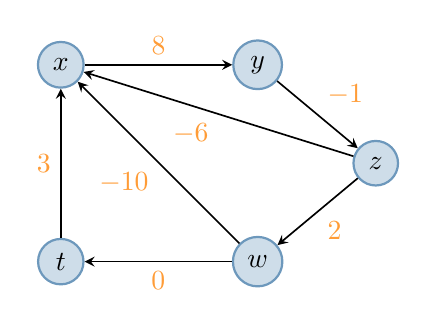
\begin{tikzpicture}[auto]

%
% Styles
%
\tikzstyle{vertex} = [circle,draw=oproverblue!60,fill=oproverblue!20,thick]
\tikzstyle{edge}   = [->,>=stealth,semithick]
\tikzstyle{weight} = [color=oproveryellow]

\node[vertex] (x) at (  1, 0)   {$x$};
\node[vertex] (y) at (3.5, 0)   {$y$};
\node[vertex] (z) at (  5,-1.25) {$z$};
\node[vertex] (w) at (3.5,-2.5)   {$w$};
\node[vertex] (t) at (  1,-2.5)   {$t$};

\draw[edge] (x) -- node[weight] {$8$}   (y);
\draw[edge] (y) -- node[weight] {$-1$}  (z);
\draw[edge] (z) -- node[weight] {$-6$}  (x);
\draw[edge] (z) -- node[weight] {$2$}   (w);
\draw[edge] (w) -- node[weight] {$-10$} (x);
\draw[edge] (w) -- node[weight] {$0$}   (t);
\draw[edge] (t) -- node[weight] {$3$}   (x);

\end{tikzpicture}


\begin{frame}
  \frametitle{Outline}
  \tableofcontents
\end{frame}

\section{Improvement for \tsolver}

\subsection{\tsolver features}

\begin{frame}
  \frametitle{\tsolver features}

\begin{itemize}

\item Incrementality: it comes for free, as we keep $\mu$ updated

\vfill\pause

\item Backtrackability: use the same trick as for BF: update
      a model $\mu'$, if satisfiable set $\mu = \mu'$, otherwise
      forget $\mu'$. When backtracking don't change $\mu$

\vfill\pause

\item Minimal \tconflicts: seen already

\vfill\pause

\item Theory Propagation:

  \begin{itemize}

    \item Bound propagation (cheap): if $x \leq c$ has been
	  asserted, then all other inactive $x \leq c'$ with
	  $c \leq c'$ are implied (similar for $\geq$)

\vfill\pause

    \item Tableau+Bound propagation: use a row
          $x_1 = a_2 x_2 + a_3 x_3 + \ldots$
	  and bounds on $x_2, x_3, \ldots$ to
	  derive bounds on $x_1$ (similar idea as to find conflicts)

  \end{itemize}

\end{itemize}

\end{frame}

\subsection{Strict inequalities}

\begin{frame}
  \frametitle{Strict inequalities}

  So far we have used bounds like $x \leq 3$, but never strict ones like $x < 3$
  \vfill\pause
  Since we are on the rationals $x < 3$ is same as $x \leq (3 - \delta)$,
  where $\delta$ is a symbolic positive parameter ($\delta > 0$) 
  \vfill\pause
  We do the following: instead of using $\Rat$ numbers of form $n$, we use $\Rat_\delta$ numbers of form $(n, k)$
  to be intended as $n + k\delta$
  \vfill\pause
  Addition in $\Rat_\delta$: $(n_1, k_1) + (n_2, k_2) = (n_1+n_2, k_1+k_2)$
  \vfill\pause
  Scalar multiplication in $\Rat_\delta$: $c(n, k) = (cn, ck)$
  \vfill\pause
  Comparison in $\Rat_\delta$: $(n_1, k_1) \leq (n_2, k_2)$ iff  ($n_1 < n_2$) or ($n_1 = n_2$ and $k_1 \leq k_2$)
  \vfill\pause
  If constraints are satisfiable, it is always possible to compute a rational 
  value for $\delta$ to translate $\Rat_\delta$ numbers into $\Rat$ numbers

\end{frame}

\begin{frame}
  \frametitle{Strict inequalities}

  \scriptsize

  Example: situation after receiving \\ 
  $x_3 < -2$, $x_4 > 0$ \\
  and after $Update(x_3,(-2,-1))$, $Update(x_4,(0,1))$

  \vfill

  \begin{columns}

  \begin{column}{.3\textwidth}
  \begin{center}
  Tableau
  \end{center}
  $$
  \begin{array}{rcl}
    x_1 & = & - x_3 + x_4  \\ 
    x_2 & = &   x_3 + x_4  \\ 
    \\
    \\
  \end{array}
  $$
  \end{column}

  \begin{column}{.4\textwidth}
  \begin{center}
  $lb$~~~~~~~Bounds~~~~~~~$ub$
  \end{center}
  $$
  \begin{array}{rcccl}
      - \infty  & \leq & x_1 & \leq & \infty \\
      - \infty  & \leq & x_2 & \leq & \infty \\
      - \infty  & \leq & x_3 & \leq & (-2,-1) \\
          (0,1) & \leq & x_4 & \leq & \infty
  \end{array}
  $$
  \end{column}

  \begin{column}{.3\textwidth}
  \begin{center}
  $\mu$
  \end{center}
  $$
  \begin{array}{rcl}
  x_1 & \mapsto &   (2,2) \\
  x_2 & \mapsto &  (-2,0) \\
  x_3 & \mapsto & (-2,-1) \\
  x_4 & \mapsto &   (0,1) 
  \end{array}
  $$
  \end{column}

  \end{columns}
  \vfill
  $x_1 = - (-2,-1) + (0,1) = (2,1) + (0,1) = (2,2)$ \\
  $x_2 =   (-2,-1) + (0,1) = (-2,0)$ 

\end{frame}

\subsection{Integers}

\begin{frame}
  \frametitle{Solving \Lia with \Lra}

  The Simplex can be used also to reason (in a complete way) about the integers (\Lia),
  e.g., using known techniques in linear programming
  \vfill
  Given a set of \Lia constraints $S$
  \begin{itemize}
    \item If $S$ is unsatisfiable 
          on \Lra\footnote{This means that we allow variables to assume values in \Rat instead of \Int.}
	  then it is also unsatisfiable on \Lia
    \item If $S$ is satisfiable on \Lra, then we have to check if there is an integer solution
  \end{itemize}
  \vfill\pause
  For the latter case the convex polytope on \Rat is explored sistematically. 
  However, in general, search is necessary: \Lia is NP-Complete, like SAT
  \begin{itemize}
    \item in SAT we split $a$ and $\neg a$, in \Lia we split $x \leq c$ and $x \geq c+1$
    \item in SAT we learn clauses, in \Lia we learn new tableau rows (new constraints)
  \end{itemize}
  \vfill\pause
  When on the integers, $\delta$ is set to $1$ ($\Rat_\delta$ numbers are not used)

\end{frame}

\begin{frame}
  \frametitle{Final Remarks}

  We did not say how to handle negative \tatoms, such as $\neg( x - y \leq c )$.
  However it is easy to see that  $\quad\neg( x - y \leq c )\quad$ iff $\quad y  - x \leq - c - 1\quad$
  \vfill
  Each \tatom is associated to two edges $(x,y;c), (y,x;-c-1)$. However
  at most only one of the two is activated (depending if \tatom is pushed positively or
  negatively)
  \vfill
  \pause
  Simple bounds, such as $\quad x \leq c\quad$ or $\quad - x \leq c\quad$ can also be handled. It is
  sufficient to add a ``fake'' (and fresh) variable $Z$ (stands for ``zero''),
  and use $\quad x - Z \leq c\quad$ and $\quad Z - x \leq c\quad$ instead of the above

\end{frame}

\begin{frame}
  \frametitle{Floyd-Warshall}

  Another algorithm that can be used instead of BF is the
  Floyd-Warshall
  \vfill
  FW has a complexity of $\theta(n^3)$, while BF of $O(nm)$
  (variations of BF have complexity $O(m + n \log n)$)
  \vfill
  FW however is useful as it is trivial to compute all
  theory propagations. In BF, theory propagations are tricky
  to discover
  \vfill
  FW is independent of $m$, the numeber of edges. FW is good
  for {\bf dense} problems, while is likely to be bad for
  {\bf sparse} ones

\end{frame}

\begin{frame}
  \frametitle{Exercizes}

  \begin{enumerate}

    \item Prove that adding $\{ (I,x_1;0), \ldots, (I,x_n;0) \}$ to a graph
          free of negative cycles, does not introduce any negative cycle

    \vfill

    \item Let $G(V,E)$ be a graph, let $x,y \in V$, and suppose that
          a path $y \rightarrow \ldots \rightarrow x$ exists in $G$.
	  Are the following true or false ? (if false, show counterexamples)

    \vfill

    \begin{enumerate}[$(a)$]

      \item Adding an edge $(x,y;100)$ to $G$ never causes the creation of a negative cycle 

      \item Adding an edge $(x,y;-100)$ to $G$ always causes the creation of a negative cycle 

    \end{enumerate}

    \vfill

    \item Let $\babst{\mu}$ be a set of constraints of the form $x - y \leq c$. Let
          $\mu$ be a model. Let $\zeta(x) = \{ \mu(x) + \epsilon \}$, 
	  for some $\epsilon \in \mathbb{Z}$. Show that $\zeta$  is also a model

    \vfill

    \item Show that conflicts returned discovered with checkNegativeCycle
          are always minimal

    \vfill

    \item Prove Observation 2 using Farka's Lemma

  \end{enumerate}

\end{frame}


\end{document}
